\documentclass[sigconf]{acmart}
\settopmatter{authorsperrow=4}
\usepackage{booktabs} % For formal tables 

\usepackage{multirow}
%\usepackage[table,xcdraw]{xcolor}
\usepackage[ruled, linesnumbered]{algorithm2e}
\usepackage{algpseudocode}

\usepackage{graphicx}
\usepackage{multirow}
\usepackage{type1cm}
\usepackage{amsmath}
\usepackage{booktabs, threeparttable}
\usepackage{color}
\usepackage{enumitem}
\usepackage{url}
\usepackage{listings}
\usepackage{subcaption}
\usepackage{caption}

\usepackage{balance} % For balanced columns on the last page

\newlist{steps}{enumerate}{1}
\setlist[steps, 1]{label = S\arabic*:}


\lstset{
  frame=tb,
  tabsize=2,
  showstringspaces=false,
  language=C++,
  basicstyle=\footnotesize,
  captionpos=b,
  keywordstyle=\color{blue},
  stringstyle=\color{red},
  numbers=left,
  xleftmargin=1em, 
  framexleftmargin=1.1em, 
  numbersep=3pt % spacing between line numbers and code
}

\def\codeinline{\lstinline[basicstyle=\small\color{darkgray},language=C++]}

%\captionsetup[table]{skip=4pt}
%\setlength{\textfloatsep}{3pt}
%\setlength{\intextsep}{2pt}

% Copyright
%\setcopyright{none}
%\setcopyright{acmcopyright}
%\setcopyright{acmlicensed}
%\setcopyright{rightsretained}
%\setcopyright{usgov}
%\setcopyright{usgovmixed}
%\setcopyright{cagov}
%\setcopyright{cagovmixed}


%\setlength{\textheight}{10.1in}
%\setlength{\textwidth}{7.8in} \setlength{\topmargin}{-0.8in}
%\setlength{\oddsidemargin}{-.62in}
%\setlength{\evensidemargin}{-.62in}

% This line disables the ACM reference format
\settopmatter{printacmref=false} 
% removes footnote with conference information in first column
\renewcommand\footnotetextcopyrightpermission[1]{} 

\begin{document}

\sloppy
%\SetAlFnt{\small}

\fancyhead{}
\title{Cpp-Taskflow: Fast Parallel Programming with Task Dependency Graphs}



\author{Chun-Xun Lin}
\affiliation{%
  \institution{Dept. of ECE, UIUC}
  \state{IL}
  \country{USA}
}
\email{clin99@illinois.edu}
%
\author{Tsung-Wei Huang}
\affiliation{%
  \institution{Dept. of ECE, UIUC}
  \state{IL}
  \country{USA}
}
\email{twh760812@gmail.com}
%
\author{Guannan Guo}
\affiliation{%
  \institution{Dept. of ECE, UIUC}
  \state{IL}
  \country{USA}
}
\email{guannan4@gmail.com}
%
\author{Martin D. F. Wong}
\affiliation{%
  \institution{Dept. of ECE, UIUC}
  \state{IL}
  \country{USA}
}
\email{mdfwong@illinois.edu}



% The default list of authors is too long for headers.
%\renewcommand{\shortauthors}{B. Trovato et al.}


\begin{abstract}
As we move to multi-core era, 
it's important for software developers to apply multi-threading to 
increase the performance of their applications.
However, parallel programming is much more difficult than writing a sequential program, 
especially when complex parallel patterns exist in the application. 
In this paper, we introduce Cpp-Taskflow \cite{cpp-taskflow}, a zero-dependency library 
written in modern C++17 to help programmers 
quickly build parallel task dependency graphs.
Cpp-Taskflow has a very neat and expressive API that allows users to master multi-threading 
in just a few minutes.
Compared with existing libraries, Cpp-Taskflow is more cost-efficient 
in performance scaling and software integration.


%is more than having multiple threads 
%executing at the same time, 
%Parallel programming is widely used in software development nowadays for 
%pursuing performance. To implement a parallel application, 


\end{abstract}


\maketitle


\section{Introduction}
\label{sec::introduction}
As a single chip accommodates more and more processing units,
parallel computing is getting increasingly important
and is no doubt a pivotal
component in building high-performance software. 
Parallel computing is also very useful for EDA applications as the recent
trend~\cite{routing}~\cite{ot}~\cite{stok}\cite{Lu2018} shows the EDA tools gain significantly speedup
by scaling to multiple cores. 
However, programming parallel applications is a very challenging task
because of difficult concurrency controls.
Immature parallelism might lead to unexpected result if one does not properly
design the control flow.  
Therefore, compared to writing sequential code, developers need to devote 
more efforts to implementing a correct parallel program.

C++ is the most widely used programming language for developing EDA
applications due to its high performance and robust standard library~\cite{cpp-thread}
in support for multi-threading.
The standard
library enables the programmers to build the parallel applications from scratch 
but it is not flexible because of low-level thread managements.
In addition to the standard library, several libraries are invented to expedite
the development of parallel program such as OpenMP~\cite{openmp} and Intel
Thread Building Blocks (TBB)~\cite{tbb}. OpenMP provides users a set of
predefined directives to annotate the desired parallelism and the compiler generates
the parallel code based on the annotations. Intel TBB is a template library that supports 
many APIs for different parallel execution patterns. Although both libraries 
solve the low-level thread management problem of standard library, they require
compiler support and library installation which causes the integration
into existing projects quite inconvenient. Furthermore, both libraries 
are not expressive in API to describe parallel applications especially
when tasks dependencies become complex.
% tbb are not expressive in API to describe parallel applications especially
% when tasks dependencies become complex

In this paper, we present Cpp-Taskflow, a header-only and zero-dependency library written in 
modern C++17. Cpp-Taskflow lets users describe the 
task dependencies in a directed acyclic graph (DAG) fasion execute tasks in parallel.
This model is very intuitive to use
and is sufficient to express most parallel execution patterns. 
The thread execution is automatically undertaken by Cpp-Taskflow and users only need to
focus on maximizing the parallelism without wrestling with the low-level thread
managements. The library is header-only which allows drop-in software integration.
In the following sections, we introduce the programming
model of Cpp-Taskflow and the associated APIs for implementing a parallel
program.



\section{Cpp-Taskflow}
From a high-level view, Cpp-Taskflow uses a DAG to represent the dependency
between tasks. A node in the DAG encapsulates a task and an edge
indicates the dependency between two tasks.  A task will be executed when all
its predecessors are executed.  Cpp-Taskflow internally employs a thread pool
to execute all tasks. 

\subsection{Static Tasking}
Listing \ref{SimpleExample} shows how to use the basic APIs of Cpp-Taskflow to create a DAG with 4 tasks.

\begin{lstlisting}[language=C++,label=SimpleExample,caption={A simple example.}]
// Cpp-Taskflow is header-only
#include <taskflow/taskflow.hpp>  

int main(){
  
  tf::Taskflow tf(4);

  // Add 4 tasks
  auto [A, B, C, D] = tf.silent_emplace(
    [] () { std::cout << "TaskA\n"; },               
    [] () { std::cout << "TaskB\n"; },               
    [] () { std::cout << "TaskC\n"; },               
    [] () { std::cout << "TaskD\n"; }                
  );                                                 
                                                     
  A.precede(B);  // B runs after A                   
  A.precede(C);  // C runs after A                   
  B.precede(D);  // D runs after B                   
  C.precede(D);  // D runs after C                   
                                                     
  tf.wait_for_all();  // block until finished

  return 0;
}
\end{lstlisting} 

First to use Cpp-Taskflow, only a single header \codeinline{taskflow.hpp} needs
to be included (line 2).  In line 6, a \codeinline{Taskflow} object
\codeinline{tf} is created with 4 threads in its thread pool. From line 9-14,
four tasks \codeinline{A, B, C, D} are added into \codeinline{tf} using the API
\codeinline{silent_emplace}.  The task dependency is annotated using the API
\codeinline{precede} from line 16-19. In line 21, the DAG is executed by
invoking the API \codeinline{wait_for_all} which blocks until all tasks finish.
In this example, task \codeinline{A} will be first executed. Then  successors
\codeinline{B} and \codeinline{C} will be executed \emph{in parallel}. Task
\codeinline{D} is the last executed.

It is clear users can easily parallelize task execution with complex dependency 
by using those concise APIs to build DAGs. Debugging parallel programs are known 
to be difficult. Cpp-Taskflow eases the burden by providing a API
\codeinline{dump} to export the DAG in Graphviz~\cite{graphviz} format. 
With the visualization capability, users can directly inspect the execution order 
to identify potential bugs.  Figure~\ref{fig::debug}
shows the dependency graph exported from Listing~\ref{DebugExample}.


\begin{lstlisting}[language=C++,label=DebugExample,caption={A debugging example.}]
#include <taskflow/taskflow.hpp>  

int main(){
  
  tf::Taskflow tf(4);  
  auto A = tf.silent_emplace([](){}).name("A");
  auto B = tf.silent_emplace([](){}).name("B");
  auto C = tf.silent_emplace([](){}).name("C");
  auto D = tf.silent_emplace([](){}).name("D");
  auto E = tf.silent_emplace([](){}).name("E");
  
  A.broadcast(B, C, E); 
  C.precede(D);
  B.broadcast(D, E); 
  
  std::cout << tf.dump();

  return 0;
}
\end{lstlisting} 

\begin{figure}[htb]
 \centering
 \includegraphics[width=.6\columnwidth]{Fig/debug.eps}
  \caption{
    The dependency graph of Listing~\ref{DebugExample}.
  }
 \label{fig::debug}
\end{figure}


\subsection{Dynamic Tasking}



\subsection{Thread Pool}


\section{ACKNOWLEDGMENT}




%\bibliographystyle{ACM-Reference-Format}
%\bibliography{sample-bibliography}

%\small 
\bibliographystyle{unsrt}
\bibliography{sigproc}  % sigproc.bib is the name of the Bibliography in this case


\end{document}
